\chapter{Taxonomy-Based Glyph Design---with a Case Study on Visualizing Workflows of Biological Experiments}


%% Uncomment below to include a teaser figure.
%  \teaser{
%  \centering
% \includegraphics[scale=.295]{images/glyph-taxonomy/bio-workflow-isacreator.eps}
% \caption{a) Workflow as rendered currently using toolkits such as GraphViz. b) We propose to replace the textual labels with glyphs, while allowing interactive access to detailed descriptions. This makes it easy to gain an overview, search components and compare workflows. The screenshot shows a prototype developed within ISAcreator, a system for capturing biological experiment metadata.}
% \label{fig:teaser}
%  }


%% Uncomment below to disable the manuscript note
%%\renewcommand{\manuscriptnotetxt}{}

%% Copyright space is enabled by default as required by guidelines.
%% It is disabled by the 'review' option or via the following command:
% \nocopyrightspace

%%%%%%%%%%%%%%%%%%%%%%%%%%%%%%%%%%%%%%%%%%% %%%%%%%%%%%%%%%%%%%%%
%%%%%%%%%%%%%%%%%%%%%% START OF THE PAPER %%%%%%%%%%%%%%%%%%%%%%


%% The ``\maketitle'' command must be the first command after the
%% ``\begin{document}'' command. It prepares and prints the title block.

%% the only exception to this rule is the \firstsection comman

\section{Introduction}
\label{sec:Introduction}
\emph{Glyph-based visualization} is a class of visual representations where a collection of small visual objects (referred to as \emph{glyphs}) are used to encode different attribute dimensions of an input data space.
A good glyph design can enable users to conduct visual search more efficiently during interactive visualization, and facilitate effective learning, memorizing and using the visual encoding scheme.
A less effective visual design may suffer from various shortcomings such as being perceptually confusing, semantically ambiguous, difficult to learn and remember, or unable to accommodate low-resolution display devices.
Most accepted designs have undergone an enduring process of evolution, refinement and standardization.
One could not and should not remove the necessity for such processes in glyph design.
Meanwhile, the design process for a glyph set usually relies on an assortment of creativity, artistic skill, domain knowledge, intuition about users, and sometimes personal preference.
While most of these qualities are absolutely helpful and some are inevitable, it is highly desirable to introduce ``systematicism'' and objectivity into the design process.

To demonstrate our approach, we elected the field of experimental biology as a test bed for developing a systematic methodology to create a glyph-based visual mapping for visualizing experimental design and experimental processes. While experimental design is at the heart of biological data evidence gathering, representation of such information is confined to either verbose description or ineffective representations. This claim is backed by a survey of public biodata repositories, devised to ensure data perennity, scientific scrutiny and reproducibility. As illustrated in Fig. \ref{fig:teaser}(a), workflows are traditionally drawn as text-based diagrams. Text labels are indices of concepts, and usually they do not encode multivariate information directly. Text-labeled boxes are costly in terms of display space usage as well as time required for visual search since parsing and interpretation of text is a slow post-attentive process \cite{ware04}. They are particularly ineffective when one needs to compare between different workflows or to identify unusual or missing components in a workflow.

Therefore, exploring an alternative in the form of glyph based representations, which are at the core of many successful schematic diagrams in the history of sciences, engineering and business management, offers a potentially more effective means for depicting these workflows.  
This presents us with an interesting case study where other types of design approaches would not be appropriate, especially in dealing with several hundreds of conceptual names.

It is important to note that domain experts are in general more willing and able to learn and memorize an encoding scheme in order to improve the accuracy and efficiency of routine tasks. At the same time, it is also necessary for an encoding scheme to facilitate effective learning and remembering through appropriate abstraction and metaphors.

Motivated by this case study, we made an observation that when a large number of concepts (or taxa) are organized into a taxonomic tree, the hierarchy typically represents an ordering of different categorization schemes.
The schemes that are higher-up in the taxonomy (closer to the root) are usually considered to be more important, which reflect their conceptual coverage, frequency of usage, domain-specific convention, and some other measurable factors.
In terms of visual encoding, higher up schemes should ideally be mapped to visual channels that have more discriminative capacity.
Hence, we can explore the parallel between the taxonomic hierarchy and the ordering of visual channels based on discriminative capacity to formulate a systematic and relatively objective process for designing a glyph set. This approach addresses one of the most common criticisms of data glyphs: the data to visual attribute mapping bias \cite{ward08}. 
Given a large data repository that encompasses many concepts, our design process is composed of four major steps:
(i) gathering and processing raw metadata for obtaining a set of taxa (names);
(ii) formulating a taxonomy based on a set of categorization schemes (Section \ref{sec:Taxonomy});
(iii) carrying out visual design, which includes the sub-process of determining the ordering of visual channels, proposing optional visual mappings, and identifying metaphoric abstractions and associations (Section \ref{sec:Glyphs}); and
(iv) implementing a glyph-based visualization system, in our case, for depicting workflows of biological experiments (Section \ref{sec:Workflow}).

Similar to most design processes, it is helpful to conduct all stages in a progressive and iterative manner.
As glyph-based visualization is normally deployed in a specific application domain, it is important to involve domain experts at every stage of the design process.
During this work, we met with domain specialists on a weekly basis.

\section{Related Work}
\label{sec:RelatedWork}
In this section, we give a brief overview of two most relevant areas in visualization, \emph{glyph-based visualization} and \emph{workflow visualization}.
The remainder background information includes the biological data management, perceptual guidance, and categorization algorithms, which will be described in the following sections where the relevant technical details are discussed.

\subsection{Glyph-based Visualization}
%
There are many examples of glyph usage in the literature spanning many disciplines, especially in conjunction with many schematic diagrams.
Bertin considered a range of simple glyphs in the context of geo-information visualization \cite{bertin83}.
Ward surveyed the use of glyphs in visualization, and discussed a number of bias issues, design approaches, and layout options \cite{ward08}.
Ropinksi \emph{et al.} conducted a survey on glyph-based techniques in medical visualizations \cite{ropinski11}.
In visualization, a number of interesting glyph designs have been presented with noticeable impact on a large range of applications (e.g., 
medicine \cite{Kindlmann06},
software \cite{Chuah98},
text \cite{Rohrer98}, and
scientific computation \cite{Wittenbrink96}).
Furthermore, Ribarsky \emph{et al.} developed an editing system, Glyphmaker \cite{ribarsky94}, to assist the process of designing glyphs.
Post \emph{et al.} proposed a language, Icon Modeling Language, for creating glyphs and glyph-style contours \cite{post95}.

There have been some recent efforts to use glyph-based visualization in biological sciences.
One noticeable attempt is the \emph{Systems Biology Graphical Notation} (SBGN) \cite{lenovere09}.
The design of SBGN makes use of the notional representations of UML with some modifications to describe the biological entities and their interactions within a biological system.
GenoCAD \cite{cai10} provides a grammar-based language for representing and searching DNA sequences and for building genetic constructs from DNA sequences, facilitating the use of conventional link diagrams.
Both systems rely heavily on text labels.
In handling a large collection of workflows, they exhibit a few shortcomings, such as inefficiency in using display space and ineffectiveness in supporting some visualization tasks, such as comparisons and novelty or anomalies detection in workflows.

In the literature, several authors encouraged glyph designers to consider visual perception when constructing glyphs \cite{ward08,karve07}. Others examined the design space of icons, which normally encode less information than glyphs (e.g., \cite{hemenway82,lewis04}). There were perceptual studies showing the merits of icons over text labels (e.g., \cite{muter86,pellegrino77}), as well as those showing the contrary (e.g., \cite{wiedenbeck99}).
Building on such discussions, this work aims to address a methodological need for a systematic approach to glyph design for applications where large collections of concepts need to be visually encoded using glyphs.

%%In \cite{ward08}, Ward summarizes that there is a need for novel mechanisms to display the growing amounts of information becoming available via the data deluge. He details the need for multi-resolution strategies \cite{ward08} giving varying levels of detail proportional to a users focus on the overall visualization.%%

\subsection{Workflow Visualization}
%
The need for \emph{workflow visualization} is pervasive across many different domains.
For example, in business and management the Gantt chart is a form of text based workflow visualization, while BPMN (Business Process Model and Notation) and EPC (Event-driven Process Chain) make use of icons to enrich text labels.
In engineering disciplines, various schematic diagrams, such as UML (Unified Modeling Language), Petri-net and circuit diagrams, are used to convey data flow and process interaction.

In this work, we consider workflows used to describe biological experiments. 
This class of workflow visualization renders the processes enacted on biological materials in an experiment (e.g., removal of blood sample from patient).
There has been little effort to develop tools that address the domain-specific needs.
Scientists usually use generic text-based graph drawing tools such as GraphViz \cite{graphviz}.

One related aspect is \emph{pathway visualization}, which is concerned with the rendering of cellular biological processes. An array of pathway visualization tools have been developed, some of which incorporate glyphs.
For example, VANTED \cite{junker06} overlays glyphs representing gene expression, enzyme and metabolite profile data on top of pathway diagrams from KEGG \cite{ogata99}.
GENeVis \cite{bourqui09}, which also employs glyphs to represent multivariate data, is a comprehensive visualization toolkit for exploration of pathways in conjunction with temporal data.
GenoCAD has at its core a workflow generation system and relies on their glyph library for rendering of the different biological processes within a cell.
SBGN-ED \cite{czauderna10}, is an add-on for the VANTED software and performs pathway creation using the aforementioned SBGN \cite{lenovere09} visual language.

%Analysis of biological data is typically a multi-stage process, involving multiple data types and sources, manipulations and algorithms.
%Graph drawing tools have been made available for bioinformaticians to keep track of these processes and to make the analysis process reproducible and sharable.
%For example, Taverna \cite{missier10} exploits color-coded boxes combined with text to indicate process type.
%KNIME \cite{berthold08} uses glyphs to indicate process types in combination with more detailed text descriptions.


%%Pathline\cite{meyer10}, a tool to visualize gene expression alongside metabolite information within particular biological pathways; 

% ====================
\section{Motivation and Overview}
\label{sec:Motivation}
%
The advent of massively parallel techniques such as DNA microarray, mass-spectrometry based proteomics and metabolomics and next generation sequencing enables molecular biologists to collect, process and manipulate biological signals on a new scale.
Big data in biology is a reality.
There has been serious effort in biology to ensure quality of experimental records by providing data archiving infrastructure and defining standards for adequate annotation and sufficient details for recapitulation of results.
A number of molecular biology signature databases have been or are being established to cover the main molecular dimensions: transcript, protein and metabolites.
The captured metadata mostly revolves around a similar configuration where sets of samples corresponding to different conditions are processed, measurements produced and analysis performed, delivering data that needs to be handled and interpreted.
While the availability of such metadata facilitates comparison across datasets and enables meta-analysis, providing means to serve an overview of experimental design can assist analysts and data managers alike, from data selection according to relevancy, to error detection such as imbalances, irregularities or inconsistencies in records.

\textbf{Task Analysis.} In the context of meta-databases for experimental records, there are two main groups of users. The majority of users are those who create data for their biological experiments or retrieve data relevant to their scientific interests. Their tasks include:
(a) entering and editing their own experimental records;
(b) transforming workflow records to schematic diagrams for comparison, external memorization, publication and education;
(c) uploading and downloading datasets;
(d) querying and searching for relevant experiments;
(e) understanding workflows of existing experimental designs;
(f) identifying similarity and difference between workflows for a common task;
(g) understand pooling events and sample relations (derivation).

The second group of users are curators who manage data archives. As biology or bioinformatics scientists themselves, they perform the above-mentioned tasks (d)-(g) frequently, and (b)-(c) occasionally. In addition, they also carry tasks for:
(h) checking syntactic correctness of submitted workflows;
(i) checking semantic correctness of submitted workflows which usually involves reading the associated publications then comparing the submitted workflows with those described in the publications;
(j) interacting with authors of submitted workflows to clarify any inconsistency and misunderstanding;
(k) making appropriate corrections in submitted records where necessary;
(l) augmenting with appropriate annotation based on additional information found in the associated publications;
(m) providing authors with submission feedback.
(n) forming an up-to-date overview about the experiments in the data archives, and maintaining an insight about the provenance of the archives;
(n) analyzing the grouping, replication, distribution and trend of experiments;
(o) analyzing ambiguities, errors and uncertainty in experimental recording, and identifying the need to enrich and refine the relevant standards for ontology, labelling and annotation.
(p) providing tools to assist users in creating meta-data from raw data.

It is not difficult to observe that effective workflow visualization can significantly improve users' capability in performing tasks b, e, f, g, h, i, j, l, n, o and p.

While it is necessary to evolve a glyph-based design for workflow visualization over a period, it is also important not to make the first step in an ad hoc manner. Such a process does not scale well with the requirements of the application concerned where a large
number of concepts are to be encoded using glyphs. We thus adopt a new systematic process for glyph design by exploring the parallel between the hierarchy of concept categorization and the ordering of discriminative capacity of visual channels. Fig. \ref{fig:workflow} depicts this process.

\begin{figure}[t!]
\centering
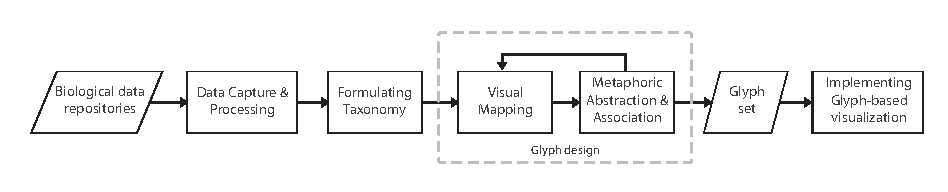
\includegraphics[scale=0.56]{images/glyph-taxonomy/workflow.eps}
\caption{A systematic process for creating glyph based representations.}
\label{fig:workflow}
\vspace{-10pt}
\end{figure}

\textbf{Data Capture and Processing}. We first retrieved workflow metadata from a biological repository (content of the ArrayExpress archive), through use of a multi-threaded harvesting operation. All experimental workflows were then converted using a MAGE-Tab to ISA-Tab converter, the latter format being more general than the former and can be used to carry metadata payloads for many types of experiments, making the data processing program more ``future-proof''.

From the 21,000 ISA-Tab files, we extracted all names of protocols (processes) and biological materials, chemical materials, devices and data used in annotation. We also computed the occurrence of each material and process found in the entire set of ISA-Tab files, which have been used as one of the metrics in the next stage (see Section 5 for details). This step results in 61 process names and 3492 names of inputs and outputs (e.g., biological and chemical materials, device measurements and data).

\textbf{Taxonomy Formulation}. Since a taxonomy for such a large collection of terms is absent, we, for starters, established a set of categorization schemes with the help of domain experts. For example, one of the schemes for categorizing processes may be based on different biological inputs to a process (e.g., molecule, cell, organism, etc.). Another scheme may be based on processing methods (e.g., perturbation, combination, etc.). We computed the quality measures of each scheme based a set of generic metrics (see Section \ref{sec:Taxonomy}) then created a taxonomic tree by recursively selecting the best categorization scheme based on the quality measures. We finalized the organization of the taxonomy by allowing domain experts (2 co-authors) to make adjustments according to domain-specific conventions. All leaf nodes of the resulting taxonomy tree are names extracted from the workflow metadata. All non-leaf nodes represent a categorization scheme.

\textbf{Glyph Design}. First, we established an ordering of commonly-used visual channels based on the literature focused on perception and visualization (see Section \ref{sec:Glyphs}). This allows us to systematically compare the order of categorization schemes in the taxonomy with the order of different visual channels. Ideally, schemes at the upper level of the tree can be mapped to visual channels which are more prominent to our visual system.

We then proceeded to the glyph design process involving two intertwined sub-processes for \textbf{visual mapping} and \textbf{metaphoric abstraction and association}. We proposed various options of visual channels for each categorization scheme featured in the taxonomic tree. We considered the merits of these visual channels and identify potential conflicts with the visual channels that have been assigned to other schemes. With the direct help from domain experts, we tried to identify a metaphoric abstraction
or association for each design option proposed. We evaluated and recorded the intuitiveness and suitability of the abstraction and metaphor association.

Informed by the results the two sub-processes, we finalized a glyph set by selecting a design option for each scheme, while maintaining the order of discriminative capacity of visual channels, minimizing conflicts between different channels, and maximizing the use of metaphoric abstraction and association.

\textbf{Implementation of Glyph-based Visualization}. We then integrated the glyph set with a layout algorithm to form a prototype system for workflow visualization (see Section \ref{sec:Workflow}). For demonstration purposes, we tested the workflow visualization in conjunction with ISAcreator, a popular domain agnostic biological experiment metadata capture tool.

% ==================
\section{Taxonomy Generation}
\label{sec:Taxonomy}

Given a large collection of concepts, we should ideally make use of a standard taxonomy, where non-leaf nodes represent different categorization schemes and each scheme provides subclasses that lead to different sub-trees. In many circumstances, however, there is no agreed taxonomic tree as establishing a standard categorization requires non-trivial scientific effort that often spans over a few decades.

The algorithm described below is not intended to establish a semantic-rich taxonomic tree for classifying concepts.
It is designed purely for addressing the needs for ordering various categorization schemes (when there is no such an agreed order) to aid glyph design, and for devising a useful tree data structure in implementing the mapping between concepts and glyphs in workflow visualization.

Hence, the criteria used for structuring the tree are based on usage of the concepts and the structural quality of the tree to be constructed.

Taxonomy is a long standing concept that can be traced back to 3000BC \cite{maguire12}. Automatic taxonomy generation has been an active field in computer science and computational biology with existing work largely focusing on clustering algorithms (e.g., \cite{krishnapuram03}). Many such algorithms assume the availability of similarity measures for ordering entities rather than relying on the existence of individual categorization schemes. In these algorithms, there is usually no attempt towards application of a metric for creating meaningful non-leaf nodes in the resulting tree. In this work, it is essential to keep each categorization scheme as a non-leaf node unless it is redundant.

\subsection{Ordering Classification Schemes}
\label{sec:Algorithm}

Let $\mathcal{X} = \{ x_{1}, x_{2}, \ldots, x_{n} \}$ be a set of concepts to be classified.
In our application, this is the set of all valid names of biological processes and IOs (inputs and outputs) in the database.
Each concept $x_i$ is associated with a scalar value, $\mu_i \in [0, 1]$, indicating its frequency of usage in relation to the total occurrence of all concepts in the database.
There are a number of categorization schemes, $\mathcal{S} = \{ S_1, S_2, \ldots, S_m \}$.
Each scheme, $S_k$ divides concepts into several classes, $c^k_1, c^k_2, \ldots, c^k_{l_k}$.
The relationship between the concept set $\mathcal{X}$ and different classification schemes can thus be represented by a Boolean matrix, $\mathbf{A}$, where each element $\alpha[i,j,k] = 1$ if concept $x_i$ belongs to the $j^{th}$ class of scheme $S_k$; otherwise $\alpha[i,j,k] = 0$.
In the context of feature-based categorization, one can also view each scheme $S_k$ as a feature, and each class under $S_k$ as a particular type of this feature.
Without losing generality, we assume that the classes under the same $S_k$ are disjoint.
It is also possible that a concept does not possess the $k^{th}$ feature, and hence does not belong to any class under $S_k$.

Given the above categorical information about the concept set $\mathcal{X}$, one can choose a categorization scheme $S_k \in \mathcal{S}$, which will divide $\mathcal{X}$ into a number of disjoint subsets corresponding to classes $c^k_1, c^k_2, \ldots, c^k_{l_k}$ and $c^k_0$.
The subset $c^k_0$ contains those concepts which $S_k$ is unable to classify.
The partitioning process can be repeated recursively by applying one of the remaining categorization schemes in $\mathcal{S}$ to each subset.
This results in a hierarchical categorization tree, which defines a taxonomy for the concepts set $\mathcal{X}$.

The ordering of the schemes in $\mathcal{S}$ thus determines the taxonomic structure of $\mathcal{X}$.
It is not difficult to anticipate that many criteria can be used to determine the ordering for a given concept set.
Some criteria will no doubt encode application-specific semantics, and some may be subjective or debatable.
However, there are also some common-sense criteria that are generic to most applications.
These include:

\textbf{Coverage}.
The number of concepts that can be classified by scheme $S_k$ is a capacity measure of $S_k$.
The more concepts that $S_k$ can classify (i.e., the fewer in $c^k_0$), the better.
The measure, which is normalized by the set size $\mid\!\mathcal{X}\!\!\mid=n$, can be defined as:

\begin{equation}
\label{eq:Coverage}
  M_1(S_k) = \frac{\sum_{i=1}^{n} \max_{1 \leq j \leq l_k} (\alpha_{i,j,k})}{n}.
\end {equation}

\textbf{Potential Usage}.
A categorization scheme that is higher up in the taxonomical tree is expected to be used more often in the application concerned.
The occurrence frequencies of concepts, $\mu_i$, enable us to estimate the potential usage of a classification scheme as follows:

\begin{equation}
\label{eq:Usage}
  M_2(S_k) = \frac{\sum_{i=1}^n \mu_i \max_{1 \leq j \leq l_k} (\alpha[i,j,k]) }
  {\sum_{i=1}^n \mu_i}.
\end {equation}

\textbf{Subtree Balance}.
Having a balanced node distribution in a tree is a desirable property of a tree structure.
It prevents a tree from having an excessive height, which corresponds to the need for more visual channels.
Let $l_k$ denote the number of subclasses in categorization scheme $S_k$,
$\tau_j$ be the number of concepts in each subclass $c^k_j, j=1, 2, \ldots, l_k$ and $\sigma_{\tau}$ and $\bar\tau$ be the standard deviation and mean respectively of $\tau_1, \ldots, \tau_{l_k}$.
We can measure the level of balance as follows:

\begin{equation}
\label{eq:Branch}
  M_3(S_k) = \begin{cases}
    0 & \sum_{i=1}^{l_{k}} \tau_{l_i} = 0 \\
    1 & \sigma_{\tau} < \epsilon (\epsilon \gt 0) \\
    P(\bar\tau \pm1 \mid N_{\bar\tau, \sigma_{\tau}}) & \bar\tau \gt 0 \; \& \;\sigma_{\tau} > \epsilon
  \end{cases}
\end {equation}

\noindent where $P$ is the probability that a value within $[\bar{\tau}-1, \bar{\tau}+1]$ falls under
the curve given by the normal distribution $N$ with $(\bar{\tau}, \sigma_\tau)$ \cite{patel96}.
There are two special cases.
When all values of $\tau_j$ are 0, $S_k$ cannot classify any concept; hence the metric returns a zero score.
When $\sigma_\tau = 0$, the subtree is totally balanced; hence the metric returns one.
As $\sigma_\tau$ approaches zero, the function $P$ becomes numerically unstable, we use a cut-off value $\epsilon$ to prevent this. In this work, we set $\epsilon = 0.00001$.
The normal distribution is preferred over a $\chi$-test, as $\chi$ may not be reliable when $l_k$ is a small number.

\textbf{Number of Subclasses}.
All visual channels used in glyphs have limited discriminative capacity.
A higher number of subclasses in a scheme would require visual encoding to have more codewords (e.g., more colors or more shape types), which will increase users' cognitive load in learning, remembering, and recognizing the codewords.
It is thus more desirable to have a smaller number of subclasses, except that a categorization scheme with fewer than 2 sub-classes is useless.
Let $\eta^{\top}$ be an up-limit for the number of codewords, which is set to 10 in this work.
We introduce the following metric to measure the discriminative capacity of a scheme:

\begin{equation}
\label{eq:Branch}
  M_4(S_k) = \begin{cases}
    0 & \eta_k < 2 \\
    \frac{\eta^{\top}-\eta_k+2}{\eta^{\top}} & 2 \leq \eta_k \leq \eta^{\top} \\
    \frac{1}{\eta^{\top}} & \eta_k > \eta^{\top}
  \end{cases}
\end {equation}

Although the above four metrics have been normalized to ensure their functional values within the $[0, 1]$ domain, the distribution of the values for different schemes can still be rather application-specific and may vary substantially between different metrics. This may lead to inconsistency in combining these metrics.

We thus provide an optional linearization filter for these metrics by mapping the values obtained using a each metric $M_i$ into fractional ranking numbers, which are then normalized into the $[0, 1]$ domain with 1 being the best and 0 the worst. For example, consider a set of six schemes with metric values:
%\[
%  (S_1, 0.5), (S_2, 0.3), (S_3, 0.5), (S_4, 0.8), (S_5, 0.8), (S_6, 0.6).
%\]
%
%\noindent We first sort the set and map the metric values to fractional ranking numbers as:
%\[
%  (S_4, 1.5), (S_5, 1.5), (S_6, 3), (S_1, 4.5), (S_3, 4.5), (S_2, 6).
%\]
%
\[
  (S_1, 0.5), (S_2, 0.3), (S_3, 0.54), (S_4, 0.8), (S_5, 0.85), (S_6, 0.6).
\]

\noindent We first sort the set:
\[
 (S_2, 0.3), (S_1, 0.5), (S_3, 0.54), (S_6, 0.6), (S_4, 0.8), (S_5, 0.85)
\]

\noindent We then obtain the normalized ranking values via the \emph{distance for ordinal variables} function $\sigma=\frac{r-1}{R-1}$ where R is the top rank and r is the rank position for each schema.
\[
  (S_2, 0), (S_1, \frac{1}{5}), (S_3, \frac{2}{5}), (S_6, \frac{3}{5}), (S_4, \frac{4}{5}), (S_5, \frac{5}{5}).
\]

We denote this filter as a function $R(S_k, M_i, \mathcal{S})$. Using the above set of metrics in conjunction with the filter $R$, we can derive a combined metric as
\[
  M(S_k) = \frac{\sum_1^4 \omega_t R(S_k, M_t(S_k), \mathcal{S})}{\sum_1^4 \omega_t}.
\]

\noindent where $\omega_t, t=1,2,3,4$ are user-adjustable weights for the four individual metrics. Similar to weights in clustering algorithms, these weights need to be used with care as they introduce additional semantics into the ordering algorithm. 

Equipped with the combined metric $M$, the algorithm for establishing an order of different schemes in $\mathcal{S}$ can be described as follows:

% TODO: Add this back in. 
%Rendering isn't completely right here... check with Min.
% \begin{program}
% \PROC select(\mathcal{S}, \mathcal{X}) \BODY
% S_{BEST} := null;  m_{BEST} := 0;
% \FOR S \in \mathcal{S} \DO
%      m := M(S);
%      \IF m > m_{BEST}
%           S_{BEST} := S;  m_{BEST} := m;
%           output(S_{BEST});
%           $remove $S_{BEST}$ from $\mathcal{S};
%           $split $\mathcal{X} $into subsets$ \mathcal{X}_{1}, \mathcal{X}_{2}, \ldots $, based on $S_{BEST};

%          \IF \mid subsets \mid \leq 1
%                return;
%         \FI
%         \FOR $each subset$ \mathcal{X}_{k} \DO
%             select(\mathcal{S}, \mathcal{X}_{i});
%        \OD
%    \FI
% \OD \ENDPROC
% \end{program}

% To illustrate our approach more clearly we present a more simple example related to classification of household items.

\subsection{Application to the Biological Case Study}
%
The biological community has built over the years a comprehensive collection of resources to archive experimental data. As molecular biology became a more data intensive field with the advent of DNA microarrays, came the need to store not only measurements but also ancillary annotation describing experimental conditions and set up, thus ensuring a metadata core always shipped with the data set. The sizes of microarray databases (GEO, AE) constitute prime resources for evaluating and testing our approach \cite{edgar02,parkinson11}. The content of ArrayExpress was therefore accessed obtaining data via parallel calls, converting 21000 experiments and associated experimental metadata to ISA-Tab\cite{rocca-serra10,sansone12}. This step provided a harmonized format in which to represent not just transcriptomic data, but also genomic, proteomic, metabolomic and other classical experiment types.

Given the data sets, the code analyzes the content of these directories to determine the processes and IOs which exist within the experiments, and the number of times they occur. The analysis revealed 61 processes (a small number resulting from the homogeneity of the database where analysis techniques are targeted primarily towards DNA microarrays) with 1,845,089 occurrences and 8,223 properties of the sample of which 3492 were deemed to be IOs with 486,353 occurrences.

Several distinct, empirical but meaningful, categorizations were devised encompassing a number of facets defining the properties of the experimental process, either in terms of its participants or in terms of key process properties. Classifications, based on features such as the nature of process participants, the granularity scale, the nature of experiments and common types a treatments applied in biological experiments were developed. Some classifications were somewhat informed by the overall assumptions ISA model relies upon, where nodes can be either material or data files and where edges are processes acting upon those nodes. Others resulted from applying a small number of axioms discovered through consultations with domain experts. There were 6 classification schemes in all with a total of 23 sub-classifications, these are detailed in figure \ref{fig:fitness-classification}. Table \ref{tab:input-fragment} shows a snapshot of the input file used in the classification algorithm.

\begin{table}[t]
\begin{center}
\caption{A fragment of the input document passed to the taxonomy generation algorithm. Schemes are grouped by common names preceding the semi-colon, e.g. \emph{S1:On Material} refers to schema 1 and \emph{On Material} is the classification.}
\vspace{1mm}
\scalebox{0.58}{

\begin{tabular}{l|ccc|c|ccc}
\textbf{Process Name} & \textbf{Occurrences} & \textbf{S1:Material} & \textbf{S1:Data} & \textbf{\ldots} & \textbf{S6:in vitro} & \textbf{S6:in vivo} & \textbf{S6:in silico}\\
\hline
\textit{labeling} & 390811 & 1 &  & \ldots & 1 &  &  \\
\textit{nucleic acid extr.} & 350267 & 1 &  & \ldots & 1 &  & \\
\textit{hybridization} & 345671 & 1 &  & \ldots & 1 &  &  \\
\textit{feature extr.} & 267044 &  & 1 & \ldots &  &  & 1 \\
\textit{bioassay data trans.} & 176347 &  & 1 & \ldots &  &  & 1 \\
\textit{grow} & 116194 & 1 &  & \ldots &  & 1 &  \\
\textit{pool} & 68004 & 1 &  & \ldots & 1 &  &  \\
\ldots & \ldots & \ldots & \ldots & \ldots & \ldots & \ldots & \ldots \\
\hline
\end{tabular}
}
\end{center}
\vspace{-5mm}
\label{tab:input-fragment}
\end{table}

The schemes are not tied to any existing taxonomic tree, may not be orthogonal and/or may be redundant with respect to others. The development of the classifications was not the result of application of any knowledge engineering methods and there is no ontological commitment, although in theory the classification names used could be derived from an ontological framework. The reason for not relying an ontology in the first place was risk mitigation, where use would almost certainly result in an unbalanced tree as occurrence counts for the terms would not be considered, resulting in creation of many glyphs that would never be used. 

\begin{figure}[ht!]
\centering
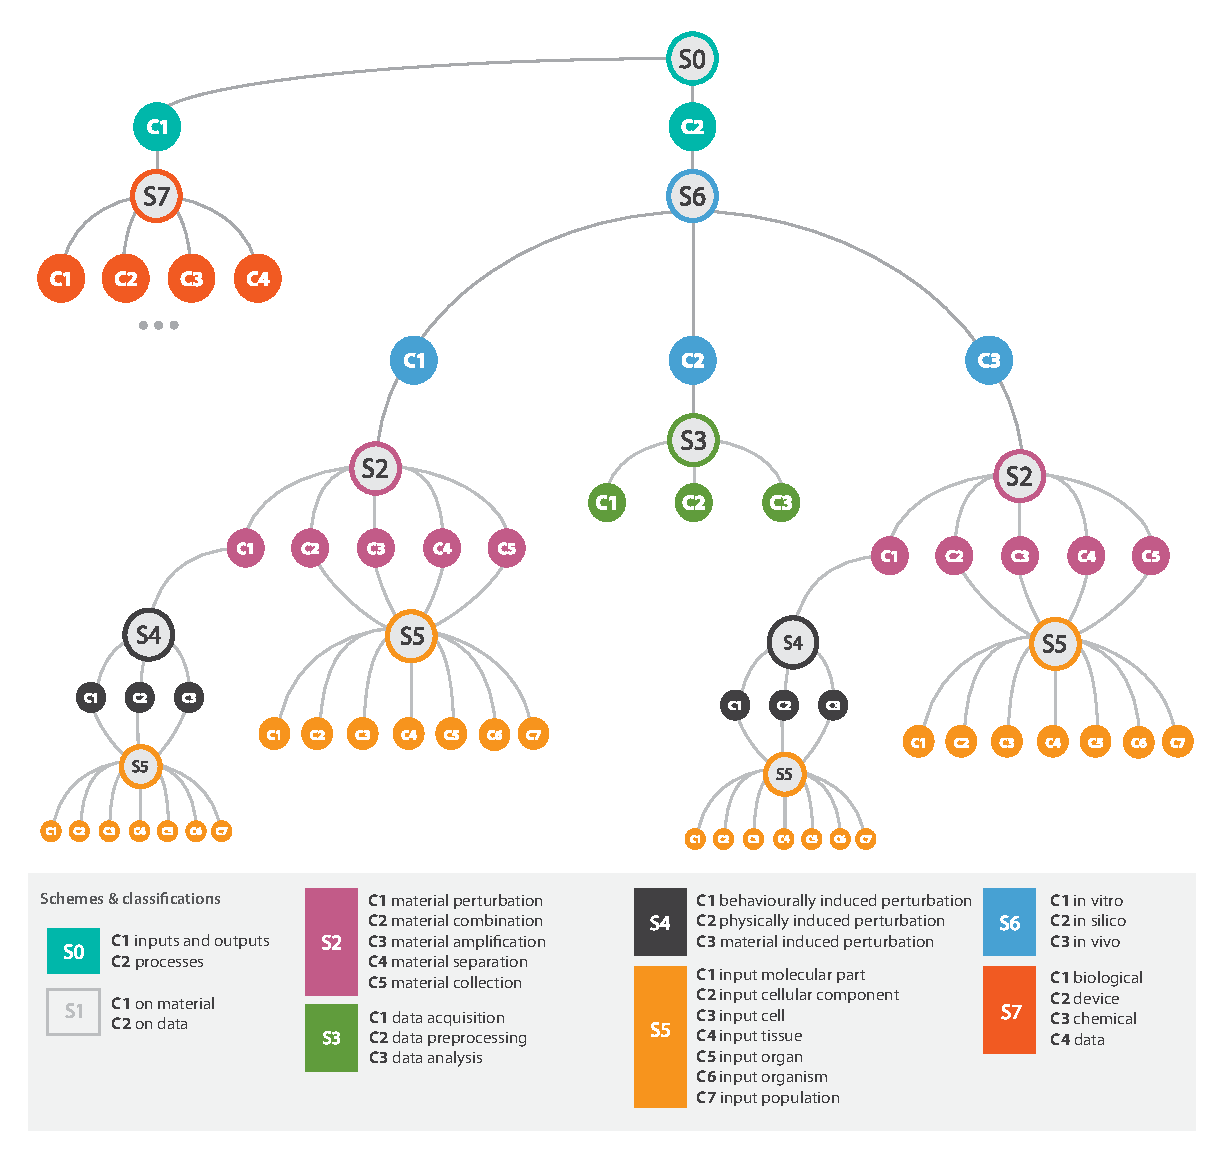
\includegraphics[scale=0.44]{images/glyph-taxonomy/fitness-classification.eps}
\caption{The classification algorithm arranged the classification schemes in the above order.}
\label{fig:fitness-classification}
\vspace{-10pt}
\end{figure}

The creation of the tree shown in Fig. \ref{fig:fitness-classification} was a largely iterative quest with continuous involvement of domain experts checking to ensure that the classifications assigned were meaningful. From early versions of the classification matrix creation, classifications were removed, added or merged in consultation with those who knew the data domain. For example, in \emph{S2} there were sub-classifications in \emph{Genetic Modification \& Labeling} which are types of \emph{Material Combination}. Therefore, these sub-classifications were removed since it would be technically and semantically incorrect to keep them. These early interactions emphasized the importance of having domain experts in the loop, otherwise classifications and subsequent glyphs would not be as well created as they could be.

The algorithm managed to correctly place the classifications where they were expected (checks were made by hand to ensure that the algorithm performed well). Schema \emph{S6} (\emph{in vitro}, \emph{in silico} and \emph{in vivo}) was the best top level classification due to its overall fitness metric of 3.08 with individual metrics found to be: M1 = 1.0; M2 = 1.0; M3 = 0.9; and M4 = 0.18. \emph{S6} was closely followed by \emph{S1} (on material and on data), however after the top level separation, \emph{S1} became redundant as a result of the top level implicitly making a split on data (in silico) and materials (in vitro and in vivo). The algorithm successfully detected this redundancy; hence $S1$ is absent from Fig. \ref{fig:fitness-classification}. 

Although the algorithm performed as expected, a possible criticism of the algorithm could be highlighted in the placement of \emph{S5} below \emph{S4}. \emph{S5} could have been placed above \emph{S4} in line with the observation that, for the majority of cases, \emph{S5} was selected over \emph{S4}. The reason \emph{S5} wasn't used to sub-classify C1 of \emph{S4} is due to its number of classifications (7) being greater than that of \emph{S4} (3), therefore \emph{S4} was selected primarily on this metric even though the sub-tree balance of \emph{S5} (0.8) was slightly better than that of \emph{S4} (0.68). To modify this behavior, it was necessary to involve domain experts in refining the tree based on their domain-specific knowledge and case-specific requirements.

% ---------------------------------------
\begin{table*}[!t]
\centering
\vspace{1mm}
\scalebox{0.67}{
\begin{tabular}{|l|l|l|l|l|l|l|c|l|c|}
\hline
 &  \textbf{Visual} & \multicolumn{ 4}{c|}{\textbf{Levels of Organization}} & \textbf{Popout} & \textbf{Hierarchy} & \textbf{Summary} & \textbf{Convention} \\
%
\textbf{Regions} & \textbf{Channels} & \textbf{Associative} & \textbf{Selective} & \textbf{Ordered} & \textbf{Quantitative} & \textbf{Effect} & \textbf{Effect} & \textbf{Strength} & \textbf{\& Metaphor} \\ \hline
%
a) Main & 1. Colour & Yes & Yes & Yes & 	& ***** & Strong  & ***** & application \\ \cline{ 2- 7}\cline{ 9- 9}
 & 2. Size &  & Yes & Yes & Yes 		& *** &   & **** &  specific \\ \cline{ 2- 7}\cline{ 9- 9}
 & 3. Shape & Yes & Yes &  &			& *** &   & *** &  \\ \cline{ 2- 7}\cline{ 9- 9}
 & 4. Orientation & Yes & Yes &  & 		& *** &   & *** & \\ \cline{ 2- 7}\cline{ 9- 9}
 & 5.Texture & Yes & Yes & Yes & 		& ** &    & ** &  \\ \cline{ 1- 9}
b) Supplementary & 6-10 (same as 1-5) &  &  &  &  &  & Medium &  & \\ \cline{ 2- 7}\cline{ 9- 9}
 & 11. Planar & Yes & Yes &  & Yes		& *** &  &  *** &  \\ \cline{ 1- 10}
c) Interior & Contains (a+b)) &  &  &  &  &				&  Low &  & \\ \hline
\end{tabular}
}
\caption{Perceptual strength of different visual channels based on levels of organization studied by Bertin\cite{Bertin:1983:book} and Green\cite{green98}, channel availability to pre-attentive processing (known as the ``popout'' effect) studied extensively in psychology \cite{williams67,duncan89,luck94,Bertin:1983:book,green98,wolfe89,treisman77,palmer77,parkhurst02}, and hierarchy effect studied by Navon \cite{navon77} and Love \cite{love99}.
The summary strength of each channel is estimated and it should be considered in conjunction with application-specific conventions and metaphors.}
\vspace{-5mm}
\label{tab:visual-variables}
\end{table*}



%\begin{table*}[t!]

\begin{center}
\scalebox{0.60}{
\begin{tabular}{|l|l|l|l|l|l|l|l|l|l|l|l|l|l|l|l|l|l|l|}
\hline
 &  & \multicolumn{ 5}{c|}{\textbf{\textit{Main}}} & \multicolumn{ 6}{c|}{\textbf{\textit{Supplementary}}} & \multicolumn{ 6}{c|}{\textbf{\textit{Interior}}} \\ \hline
 &  & \textbf{Colour} & \textbf{Size} & \textbf{Shape} & \textbf{Orientation} & \textbf{Texture} & \textbf{Colour} & \textbf{Size} & \textbf{Shape} & \textbf{Orientation} & \textbf{Texture} & \textbf{Planar} & \textbf{Colour} & \textbf{Size} & \textbf{Shape} & \textbf{Orientation} & \textbf{Texture} & \textbf{Planar} \\ \hline
\multicolumn{ 1}{|l|}{\textbf{\textit{Main}}} & \textbf{Colour} & \cellcolor{Gray} & $\gt$\cellcolor{Orange} \cite{williams67,luck94} & $\gt$\cellcolor{Orange} \cite{williams67} & $\gt$\cellcolor{Orange} \cite{luck94, parkhurst02} & Unk\cellcolor{Cream} & $\gt$\cellcolor{Orange} & $\gt$\cellcolor{Orange} & $\gt$\cellcolor{Orange} & $\gt$\cellcolor{Orange} & Unk\cellcolor{Cream} & Unk\cellcolor{Cream} & $\gt$\cellcolor{Orange} & $\gt$\cellcolor{Orange} & $\gt$\cellcolor{Orange} & $\gt$\cellcolor{Orange} & Unk\cellcolor{Cream} & Unk\cellcolor{Cream} \\ \cline{ 2- 19}
\multicolumn{ 1}{|l|}{} & \textbf{Size} & $\lt$\cellcolor{Blue} & \cellcolor{Gray} & $\gt$\cellcolor{Orange} \cite{williams67} & $\gt$\cellcolor{Orange} \cite{williams67,luck94} & Unk\cellcolor{Cream} & $\gt$\cellcolor{Orange} & $\gt$\cellcolor{Orange} & $\gt$\cellcolor{Orange} & $\gt$\cellcolor{Orange} & Unk\cellcolor{Cream} & Unk\cellcolor{Cream} & $\gt$\cellcolor{Orange} & $\gt$\cellcolor{Orange} & $\gt$\cellcolor{Orange} & $\gt$\cellcolor{Orange} & Unk\cellcolor{Cream} & Unk\cellcolor{Cream} \\ \cline{ 2- 19}
\multicolumn{ 1}{|l|}{} & \textbf{Shape} & $\lt$\cellcolor{Blue} & $\lt$\cellcolor{Blue} & \cellcolor{Gray} & $\gt$ \cite{luck94}\cellcolor{Orange} & Unk\cellcolor{Cream} & $\gt$\cellcolor{Orange} & $\gt$\cellcolor{Orange} & $\gt$\cellcolor{Orange} & $\gt$\cellcolor{Orange} & Unk\cellcolor{Cream} & Unk\cellcolor{Cream} & $\gt$\cellcolor{Orange} & $\gt$\cellcolor{Orange} & $\gt$\cellcolor{Orange} & $\gt$\cellcolor{Orange} & Unk\cellcolor{Cream} & Unk\cellcolor{Cream} \\ \cline{ 2- 19}
\multicolumn{ 1}{|l|}{} & \textbf{Orientation} & $\lt$\cellcolor{Blue} & $\lt$\cellcolor{Blue} & $\lt$\cellcolor{Blue} & \cellcolor{Gray} & Unk\cellcolor{Cream} & $\gt$\cellcolor{Orange} & $\gt$\cellcolor{Orange} & $\gt$\cellcolor{Orange} & $\gt$\cellcolor{Orange} & Unk\cellcolor{Cream} & Unk\cellcolor{Cream} & $\gt$\cellcolor{Orange} & $\gt$\cellcolor{Orange} & $\gt$\cellcolor{Orange} & $\gt$\cellcolor{Orange} & Unk\cellcolor{Cream} & Unk\cellcolor{Cream} \\ \cline{ 2- 19}
\multicolumn{ 1}{|l|}{} & \textbf{Texture} & Unk\cellcolor{Cream} & Unk\cellcolor{Cream} & Unk\cellcolor{Cream} & Unk\cellcolor{Cream} & \cellcolor{Gray} & Unk\cellcolor{Cream} & Unk\cellcolor{Cream} & Unk\cellcolor{Cream} & Unk\cellcolor{Cream} & $\gt$\cellcolor{Orange} & Unk\cellcolor{Cream} & Unk\cellcolor{Cream} & Unk\cellcolor{Cream} & Unk\cellcolor{Cream} & Unk\cellcolor{Cream} & $\gt$\cellcolor{Orange} & Unk\cellcolor{Cream} \\ \hline
\multicolumn{ 1}{|l|}{\textbf{\textit{Supplementary}}} & \textbf{Colour} & $\lt$\cellcolor{Blue} & $\lt$\cellcolor{Blue} & $\lt$\cellcolor{Blue} & $\lt$\cellcolor{Blue} & Unk\cellcolor{Cream} & \cellcolor{Gray} & $\gt$\cellcolor{Orange} & $\gt$\cellcolor{Orange} & $\gt$\cellcolor{Orange} & Unk\cellcolor{Cream} & Unk\cellcolor{Cream} & $\gt$\cellcolor{Orange} & $\gt$\cellcolor{Orange} & $\gt$\cellcolor{Orange} & $\gt$\cellcolor{Orange} & Unk\cellcolor{Cream} & Unk\cellcolor{Cream} \\ \cline{ 2- 19}
\multicolumn{ 1}{|l|}{} & \textbf{Size} & $\lt$\cellcolor{Blue} & $\lt$\cellcolor{Blue} & $\lt$\cellcolor{Blue} & $\lt$\cellcolor{Blue} & Unk\cellcolor{Cream} & $\lt$\cellcolor{Blue} & \cellcolor{Gray} & $\gt$\cellcolor{Orange} & $\gt$\cellcolor{Orange} & Unk\cellcolor{Cream} & Unk\cellcolor{Cream} & $\gt$\cellcolor{Orange} & $\gt$\cellcolor{Orange} & $\gt$\cellcolor{Orange} & $\gt$\cellcolor{Orange} & Unk\cellcolor{Cream} & Unk\cellcolor{Cream} \\ \cline{ 2- 19}
\multicolumn{ 1}{|l|}{} & \textbf{Shape} & $\lt$\cellcolor{Blue} & $\lt$\cellcolor{Blue} & $\lt$\cellcolor{Blue} & $\lt$\cellcolor{Blue} & Unk\cellcolor{Cream} & $\lt$\cellcolor{Blue} & $\lt$\cellcolor{Blue} & \cellcolor{Gray} & $\gt$\cellcolor{Orange} & Unk\cellcolor{Cream} & Unk\cellcolor{Cream} & $\gt$\cellcolor{Orange} & $\gt$\cellcolor{Orange} & $\gt$\cellcolor{Orange} & $\gt$\cellcolor{Orange} & Unk\cellcolor{Cream} & Unk\cellcolor{Cream} \\ \cline{ 2- 19}
\multicolumn{ 1}{|l|}{} & \textbf{Orientation} & $\lt$\cellcolor{Blue} & $\lt$\cellcolor{Blue} & $\lt$\cellcolor{Blue} & $\lt$\cellcolor{Blue} & Unk\cellcolor{Cream} & $\lt$\cellcolor{Blue} & $\lt$\cellcolor{Blue} & $\lt$\cellcolor{Blue} & \cellcolor{Gray} & Unk\cellcolor{Cream} & Unk\cellcolor{Cream} & $\gt$\cellcolor{Orange} & $\gt$\cellcolor{Orange} & $\gt$\cellcolor{Orange} & $\gt$\cellcolor{Orange} & Unk\cellcolor{Cream} & Unk\cellcolor{Cream} \\ \cline{ 2- 19}
\multicolumn{ 1}{|l|}{} & \textbf{Texture} & Unk\cellcolor{Cream} & Unk\cellcolor{Cream} & Unk\cellcolor{Cream} & Unk\cellcolor{Cream} & Unk\cellcolor{Cream} & Unk\cellcolor{Cream} & Unk\cellcolor{Cream} & Unk\cellcolor{Cream} & Unk\cellcolor{Cream} & \cellcolor{Gray} & Unk\cellcolor{Cream} & Unk\cellcolor{Cream} & Unk\cellcolor{Cream} & Unk\cellcolor{Cream} & Unk\cellcolor{Cream} & $\gt$\cellcolor{Orange} & Unk\cellcolor{Cream} \\ \cline{ 2- 19}
\multicolumn{ 1}{|l|}{} & \textbf{Planar} & Unk\cellcolor{Cream} & Unk\cellcolor{Cream} & Unk\cellcolor{Cream} & Unk\cellcolor{Cream} & Unk\cellcolor{Cream} & Unk\cellcolor{Cream} & Unk\cellcolor{Cream} & Unk\cellcolor{Cream} & Unk\cellcolor{Cream} & Unk\cellcolor{Cream} & \cellcolor{Gray} & Unk\cellcolor{Cream} & Unk\cellcolor{Cream} & Unk\cellcolor{Cream} & Unk\cellcolor{Cream} & Unk\cellcolor{Cream} & Unk\cellcolor{Cream} \\ \hline
\multicolumn{ 1}{|l|}{\textbf{\textit{Interior}}} & \textbf{Colour} & $\lt$\cellcolor{Blue} & $\lt$\cellcolor{Blue} & $\lt$\cellcolor{Blue} & $\lt$\cellcolor{Blue} & Unk\cellcolor{Cream} & $\lt$\cellcolor{Blue} & $\lt$\cellcolor{Blue} & $\lt$\cellcolor{Blue} & $\lt$\cellcolor{Blue} & Unk\cellcolor{Cream} & Unk\cellcolor{Cream} & \cellcolor{Gray} & $\gt$\cellcolor{Orange} & $\gt$\cellcolor{Orange} & $\gt$\cellcolor{Orange} & Unk\cellcolor{Cream} & Unk\cellcolor{Cream} \\ \cline{ 2- 19}
\multicolumn{ 1}{|l|}{} & \textbf{Size} & $\lt$\cellcolor{Blue} & $\lt$\cellcolor{Blue} & $\lt$\cellcolor{Blue} & $\lt$\cellcolor{Blue} & Unk\cellcolor{Cream} & $\lt$\cellcolor{Blue} & $\lt$\cellcolor{Blue} & $\lt$\cellcolor{Blue} & $\lt$\cellcolor{Blue} & Unk\cellcolor{Cream} & Unk\cellcolor{Cream} & $\lt$\cellcolor{Blue} & \cellcolor{Gray} & $\gt$\cellcolor{Orange} & $\gt$\cellcolor{Orange} & Unk\cellcolor{Cream} & Unk\cellcolor{Cream} \\ \cline{ 2- 19}
\multicolumn{ 1}{|l|}{} & \textbf{Shape} & $\lt$\cellcolor{Blue} & $\lt$\cellcolor{Blue} & $\lt$\cellcolor{Blue} & $\lt$\cellcolor{Blue} & Unk\cellcolor{Cream} & $\lt$\cellcolor{Blue} & $\lt$\cellcolor{Blue} & $\lt$\cellcolor{Blue} & $\lt$\cellcolor{Blue} & Unk\cellcolor{Cream} & Unk\cellcolor{Cream} & $\lt$\cellcolor{Blue} & $\lt$\cellcolor{Blue} & \cellcolor{Gray} & $\gt$\cellcolor{Orange} & Unk\cellcolor{Cream} & Unk\cellcolor{Cream} \\ \cline{ 2- 19}
\multicolumn{ 1}{|l|}{} & \textbf{Orientation} & $\lt$\cellcolor{Blue} & $\lt$\cellcolor{Blue} & $\lt$\cellcolor{Blue} & $\lt$\cellcolor{Blue} & Unk\cellcolor{Cream} & $\lt$\cellcolor{Blue} & $\lt$\cellcolor{Blue} & $\lt$\cellcolor{Blue} & $\lt$\cellcolor{Blue} & Unk\cellcolor{Cream} & Unk\cellcolor{Cream} & $\lt$\cellcolor{Blue} & $\lt$\cellcolor{Blue} & $\lt$\cellcolor{Blue} & \cellcolor{Gray} & Unk\cellcolor{Cream} & Unk\cellcolor{Cream} \\ \cline{ 2- 19}
\multicolumn{ 1}{|l|}{} & \textbf{Texture} & Unk\cellcolor{Cream} & Unk\cellcolor{Cream} & Unk\cellcolor{Cream} & Unk\cellcolor{Cream} & Unk\cellcolor{Cream} & Unk\cellcolor{Cream} & Unk\cellcolor{Cream} & Unk\cellcolor{Cream} & Unk\cellcolor{Cream} & $\lt$\cellcolor{Blue} & Unk\cellcolor{Cream} & Unk\cellcolor{Cream} & Unk\cellcolor{Cream} & Unk\cellcolor{Cream} & Unk\cellcolor{Cream} & \cellcolor{Gray} & Unk\cellcolor{Cream} \\ \cline{ 2- 19}
\multicolumn{ 1}{|l|}{} & \textbf{Planar} & Unk\cellcolor{Cream} & Unk\cellcolor{Cream} & Unk\cellcolor{Cream} & Unk\cellcolor{Cream} & Unk\cellcolor{Cream} & Unk\cellcolor{Cream} & Unk\cellcolor{Cream} & Unk\cellcolor{Cream} & Unk\cellcolor{Cream} & Unk\cellcolor{Cream} & Unk\cellcolor{Cream} & Unk\cellcolor{Cream} & Unk\cellcolor{Cream} & Unk\cellcolor{Cream} & Unk\cellcolor{Cream} & Unk\cellcolor{Cream} & \cellcolor{Gray} \\ \hline
\end{tabular}


}
\end{center}
\caption{Comparison of selected retinal variables available for the glyph design and their expected priority interactions based on review of effects presented in Table 1.
Unk. Unknown: no data documenting the interaction. > superiority/precedence , < inferiority/deference where row value are on the left of the operator and column value is the right term of the the operator.}
\label{tab:visual-variable-strength}
\end{table*}


% ==============
\section{Visual Encoding}
\label{sec:Glyphs}
\subsection{Perceptual Guidance}
%
A \emph{glyph} is a small visual object composed of a number of \emph{visual channels} which can be used independently as well as constructively to depict attributes of a data record.
Glyphs are of a type of visual signs that can make use of visual features of other types of signs, such as icons, indices and symbols.

Although there are several books on sign design (e.g., \cite{barker00,abdullah06}), they focus on signage in public space, and offer empirical guidance on a large number of issues including standardization, size, location, illumination and so on.
Many of these issues are not quite relevant to the need for visualizing the workflows of biological experiments. Here, we draw our design principles mainly from findings in perception, especially in the area of visual search \cite{spoehr82,quinlan03}.

While the extensive use of signs, icons and pictograms in everyday life reflects their usefulness and effectiveness, several perceptual studies also directly or indirectly confirmed their perceptual and cognitive merits.
For example, Franks and Bransford's study on transformation of prototypes \cite{franks71} suggested that humans can learn to recognize glyphs by rules consciously as well as unconsciously.
The presence of iconic memory \cite{sperling60} may facilitate rapid comparison between glyphs in the same display, whereas it is less so for texts.

\textbf{Guideline on Semantic Relevance}.
Bertin \cite{bertin83} classified visual channels (which he referred to as retinal variables) into two categories, planar (location) and retinal (size, color, shape, orientation, texture and brightness).
Bertin proposed four semantic criteria for determining the suitability of different channels in representing certain types of information.
These semantic criteria are: \emph{associative}, \emph{selective}, \emph{ordered} and \emph{quantitative}.
These criteria are important guidelines, though there has been disagreement in the literature as to how individual visual channels are judged.
For example, Bertin considered shape as a non-selective variable.
Research has shown that shapes such as filled rectangles, circles and triangles do not allow the human visual system to identify one shape from another effectively in a rapid action when they form some global structures \cite{love99, navon77}, (they have poor ``pop-out'' effect).
However, the omission of all shapes as a selective visual channel has been challenged, for example, by \cite{treisman88,wang94,green98}, who show practice and familiarity can support selectivity with almost any shape.

\textbf{Guideline on Channel Composition}.
As a glyph is likely to feature a number of visual channels, the constructive composition may affect how individual channels are perceived.
A rich collection of literature on integral and separable dimensions shows that the combined dissimilarity of closely integrated visual channels exhibits Euclidean distance $\sqrt{d^2_a + d^2_b}$ \cite{krantz75,handelt72}, whereas that of separable visual channels exhibits city-block distance $d_a  + d_b$ \cite{burns78,shepard64}. 
The latter is more cost-effective than the former in rule-based encoding of multi-faceted concepts, therefore effective glyph design should encompass a non-conflicting set of separable retinal variables. 

\textbf{Guideline on Pop-out Effects}.
Many classic studies in perception also established the ``power'' of different visual channels in terms of \emph{pop-out effect} (pre-attentive search), and fixation (during attentive search)\cite{healey11}.
The \emph{pop-out effect} is one which allows identification of a target within a few nanoseconds of initial exposure to the visual search space.
A result of several milestone studies focusing on observed response times, the ordering of the four commonly used visual channels follows the consensus: color $\prec$ size $\prec$ shape $\prec$ orientation (e.g.,\cite{williams67,quinlan97,ropinski11}).
The symbol $\prec$ reads as \emph{precedes}. However, the strength of color over the other three channels is generally much more noticeable. 

\textbf{Guideline on Visual Hierarchy}.
%
\emph{Visual hierarchy}, with which the environment and objects around us are arranged is a well documented theoretical framework \cite{palmer77,navon77, love99, kinchla79,bar04}.
However, the literature contains a debate over the ways in which the visual system traverses this hierarchy.
There are four possible ways:
top-down (also called global processing) \cite{navon77};
bottom-up (also called local processing);
middle-out \cite{kinchla79};
and salient features (\emph{e.g., edges, points, colors}) \cite{rumelhart70}.
Because glyphs are relatively small in comparison with a whole visualization, we consider at such a ``localized level'', the top-down and salient features may play more significant roles.
The top-down assumption suggests that when consider a glyph in isolation, its global feature will affect visual search more than its local features.
Salient features are partly addressed by the pop-out effects.

\begin{figure}[t]
\centering
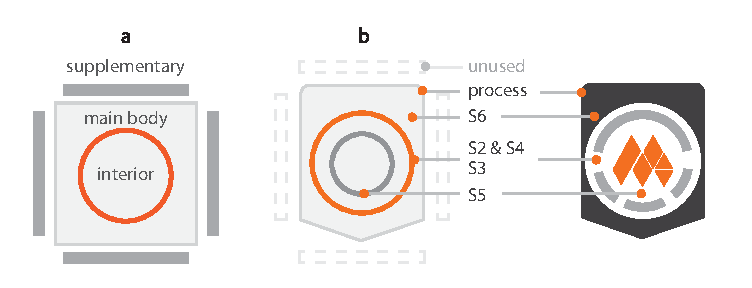
\includegraphics[width=86mm]{images/glyph-taxonomy/glyph-space.eps}
\caption{(a) The glyph template with a main body, an interior region and an exterior region (consisting of 4 sections).
(b) Our final design makes use of the main body and interior region.
The exterior is reserved for future extension.
% As we proceed to lower levels, size will have an impact on visual power\cite{duncan89}.
}
\label{fig:glyph-design}
\vspace{-10pt}
\end{figure}

Based on the above-mentioned perceptual guidance, we considered a generic glyph design template for this work as shown in Fig. \ref{fig:glyph-design}(a).
The template divides a glyph into three regions, namely \emph{main body}, \emph{exterior} and \emph{interior}.
In practice, each region can be divided into 2 or more sub-regions (e.g., a twin body glyph or 4 exterior sections), it is convenient to consider the three regions in abstraction.
The separation of these regions facilitates the basic separation of visual channels based on the composition guideline, while allowing us to consider them individually according to the hierarchy guideline.

In theory, the exterior and interior regions may also be divided into sub-regions in a recursive fashion though in practice this is tightly constrained or discouraged by the very limited display resolution typically available for glyphs.
Similar to the design convention for icons, pictograms are normally featured in the interior region.
The exterior region may be further divided in four sections (top, bottom, left and right).
If glyphs will be connected to form a network or graph (as in this work), the use of these four sections has to take into account the possible incoming and outgoing connections.

Table \ref{tab:visual-variables} summarizes relative merits of some of the most commonly-used visual channels in different regions according to Bertin's categorization, pop-out effects and hierarchy effects.
We estimated the overall discriminating capacity of each channel by using a summary rating in the penultimate column.
We also recognized the importance of the conventions and metaphors in an application.
We will discuss visual metaphors further in Section \ref{sec:Mapping}.
We added the last column to highlight the necessity to consider these in a design process.

It is difficult to establish an accurate ranking order of different visual channels by taking all perceptual effects into account in a quantitative manner.
The state of the art in perception research is yet to provide all evidence needed for a full and conclusive analysis.
Nevertheless, Table \ref{tab:visual-variables} can serve a qualitative guidance to glyph designs in this work, providing an ordering of visual channels in parallel with the ordering of categorization schemes discussed in Section \ref{sec:Taxonomy}.

% ---------------------------------------------------------
\subsection{Mapping Taxonomy to Visual Channels}
\label{sec:Mapping}

For each scheme in the taxonomic tree as shown in Fig. \ref{fig:fitness-classification}, we propose a number of design options.
Fig. \ref{fig:design-options} shows some examples of the proposed designs.
For example, the first column shows the use of colors to encode the classes of a categorization scheme.
The second column shows the use abstract shapes.
Some options convey an abstraction from pictorial representations of classes, and in other cases, we try to establish a metaphoric association between a visual channel and a biological categorization. 

Metaphoric visual representations enable domain-specific encoding using ``natural mapping'' \cite{siirtola05,norman02}. This natural mapping can make it easier for users to infer meaning from the glyph with less effort required to learn and remember them \cite{McDougall00}.
A recent study showed that visual metaphors can aid memorization of the information depicted in a visualization \cite{Borgo12}. However, the same study also showed that visually realistic metaphors 
(those with a lot of detail) may have a negative impact on performance in visual search. Moreover, realistic visual metaphors require a higher pixel resolution, and would lose their discriminating capacity in low resolution conditions. 

\begin{figure}[t!]
\centering
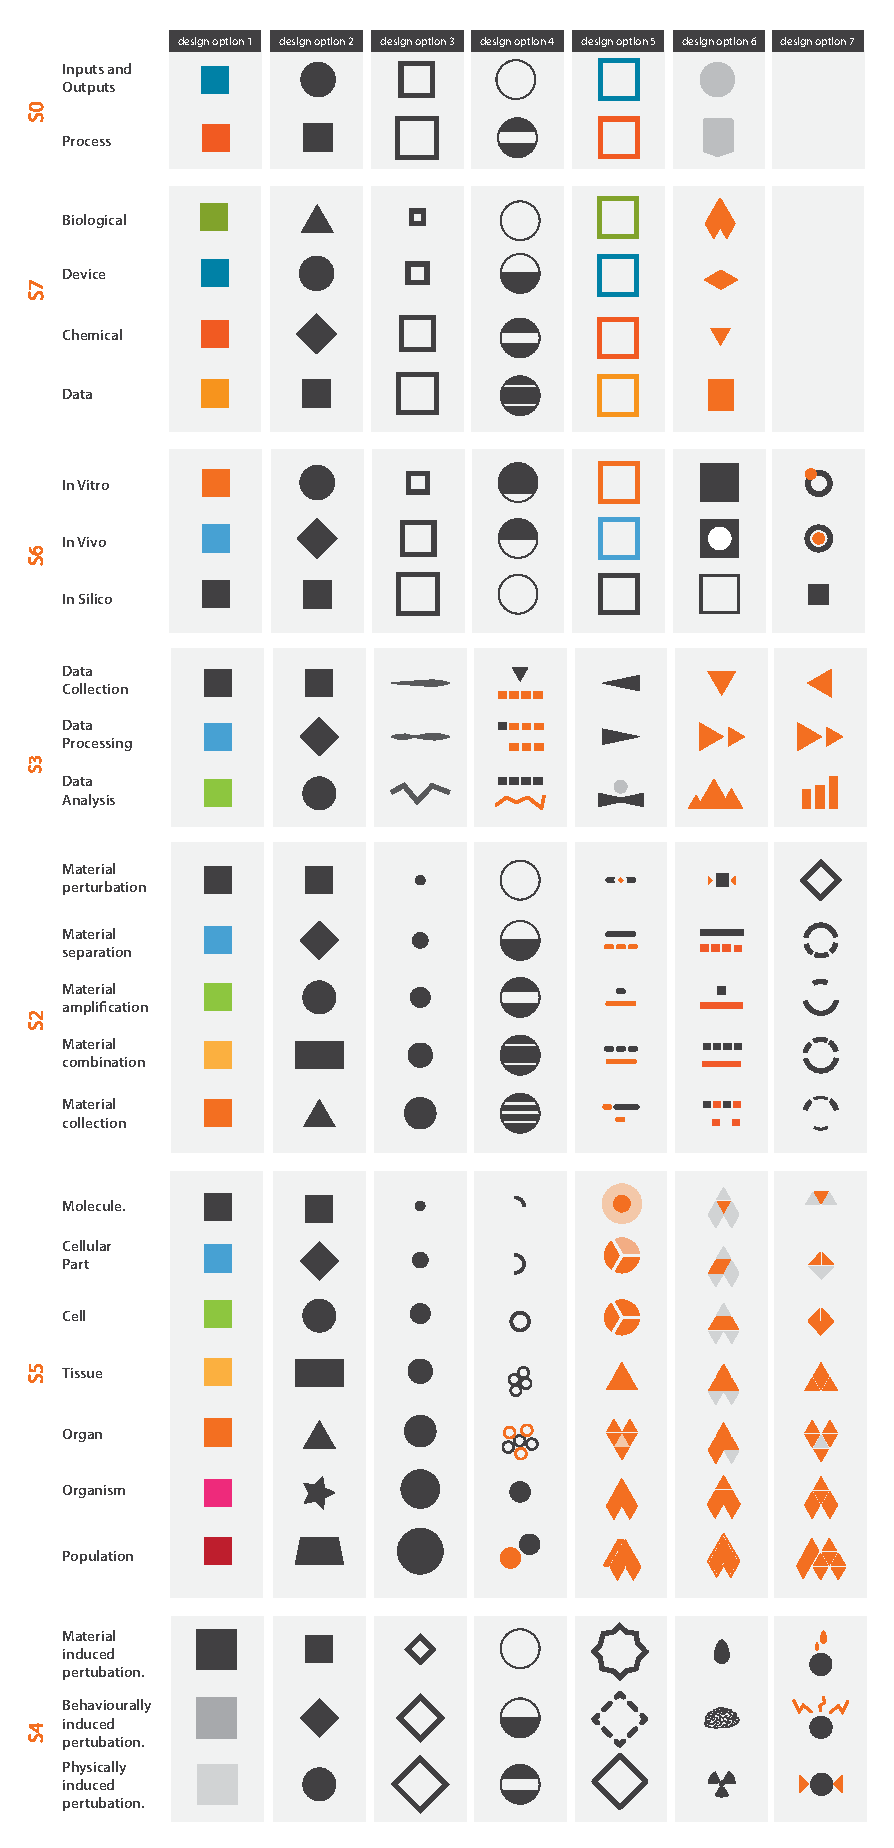
\includegraphics[scale=0.605]{images/glyph-taxonomy/design-options.eps}
\caption{Experimenting with visual channels: an overview of the various design options available for use in representing the different classifications. Most schemes for IO categorization are not shown due to space restriction.}
\label{fig:design-options}
\vspace{-10pt}
\end{figure}

Based on the design options shown in Fig. \ref{fig:design-options}, we followed the taxonomic tree in Fig. \ref{fig:fitness-classification} and identified the best option for each scheme in a hierarchical manner.
The evaluation criteria include:
%
\begin{itemize}
\vspace{-1mm}
\item
the discriminating capacities of different channels (Table \ref{tab:visual-variables});
\vspace{-2mm}
\item
metaphoric capacity for aiding learning and remembering;
\vspace{-2mm}
\item
potential conflicts, including spatial, perceptual and metaphoric conflicts, with visual channels that have already been assigned to other schemes in the tree;
\vspace{-2mm}
\item
encoding costs in terms of requirement for pixel resolution.
\end{itemize}

This process normally takes a few iterations, during which new design options and new metaphoric abstractions and associations are sometimes proposed.

\begin{figure}[t!]
\centering
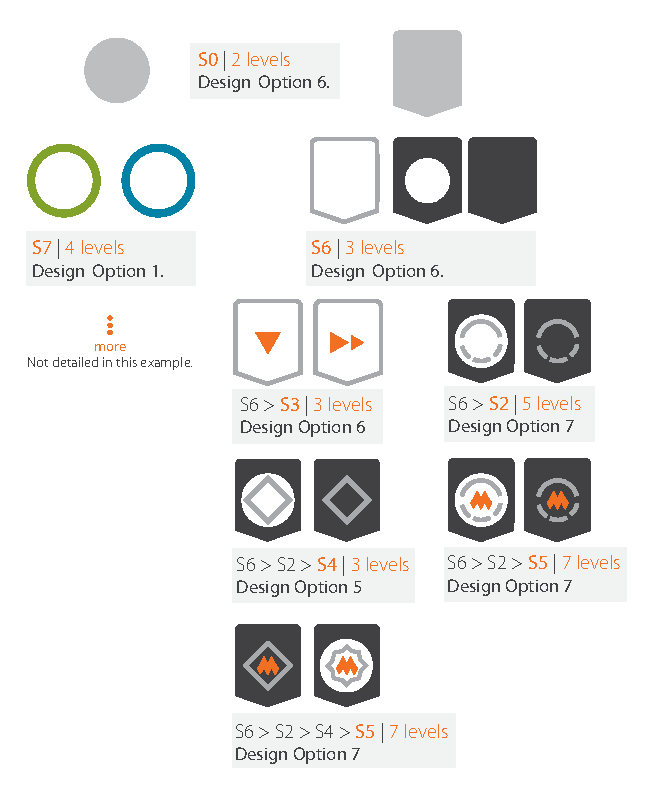
\includegraphics[scale=0.7]{images/glyph-taxonomy/glyph-design-selection.eps}
\caption{Formation of the final glyph design. Top level items require the greatest visual power. It is important to be able to distinguish each of the processes based on their parent level in the taxonomy. Distinguishable global shapes provide the difference between IOs (circles) and processes (squares with pointed bottom to indicate directionality).}
\label{fig:glyph-design-selection}
\vspace{-10pt}
\end{figure}

Based on the hierarchy in Fig. \ref{fig:fitness-classification}, we considered to use color and shape options for S0 (IOs vs. processes) and S7 (four classes of IOs).
As introducing 4 main body shapes to encode IOs is not an effective mapping for learning and remembering, we decided to assign outline color of the main body to encode S7, and use two basic shapes, circle and pentagon (a rectangle with a pointer to show workflow direction) to encode S0.
Since the main body or the pentagon will only be colored in black or white, S0 also implicitly encoded in using color symbolism, that is, color for IOs and black/white for processes.
In effect, S0 is encoded using two visual channels.
This redundancy can serve as an error detection in visualization \cite{Chen10}.

Fig. \ref{fig:glyph-design-selection} shows each of the five schemes for the process subtree, and the design option chosen from Fig. \ref{fig:design-options}.
Below we discuss our reasoning for selecting each of the design options for each scheme in the taxonomy.


\textbf{S6: Process environment}.
The taxonomic tree suggested a high priority for visual mapping, which is consistent with the domain experts' intuition.
We took advantage that black color was not used by S7 for IOs, we assigned a white background to \emph{in silico/in computer} (related to computational processes), and black to \emph{in vivo/in living)}  and \emph{in vitro/in glass} (related to materials).
Further more, we made use of a shape-based metaphor, fully-filled background for \emph{in vivo} (whole organism), and black background with white cut out for \emph{in vitro} (component of an organism).
Together, this was given in Fig. \ref{fig:design-options} as design option 6.
We maintained the overall appearance of the main body of process glyphs in black and white to avoid potential clash with material glyphs.

\textbf{S2: Types of Material Manipulation}.
S2 has 5 classes, and we adopted design option 7, which employs visual metaphors that encapsulate strong domain-specific meanings.
For example, visual symbol for the \emph{material amplification} class depicts a small segment becoming a large segment.

\textbf{S4: Type of Experimental Perturbation}.
S4 defines 3 further sub-classes of the \emph{material perturbation} class of S2.
Due to the low number of subclasses, we made use of line styles to modify the diamond shape of the \emph{material perturbation}.
We made metaphoric association of three line styles as:
``solid'' line for physically induced perturbation;
dash line, a common metaphor for uncertainty and unpredictability, for behaviorally induced perturbation; and
wavy line, which is closer to a circle (a visual signature for IOs), for material induced perturbation.

\textbf{S5: Levels of Material Granularity}.
This scheme has 7 subclasses (molecule, cellular part, cell, tissue, organ, organism and population), and finding a suitable visual channel was not straightforward. A simplest approach would be to use colors to fill the interior of the glyph, or to use some shape-based encoding.
After consulting the domain experts, these two options were ruled out.
In fact, domain experts preferred some pictograms to represent the 7 subclasses.
After considering a number of more realistic drawings, we found that it was not easy to create realistic representations that can differentiate all subclasses (e.g., cellular part vs. cell; organ vs. organism).
We designed a special set of icons as shown in Fig. \ref{fig:s5-metaphor} with three visual channels to aid learning, memorization and recognition.
The first visual channel is the overall shape and orientation.
The second visual channel is metaphoric abstraction and association.
For example, the shape of cell part indicates a portion of a cell.
Tissue is associated with a patch, organ with an abstract heart shape, organism with an abstract human, population with two abstract humans.
The third visual channel is the number of orange sub-shapes, representing the levels 1-7.
\begin{figure}[t!]
\centering

\includegraphics[scale=1]{images/glyph-taxonomy/s5-metaphor.eps}
\caption{Visual representations of the 7 classes in \emph{S5}.}
\label{fig:s5-metaphor}
\vspace{-10pt}
\end{figure}

\textbf{S3: Types of Data Manipulation}.
S3 defines a 3 further sub-classes of the \emph{in silico} class of S6.
We use three abstract pictograms to represent data capture, processing and analysis. The encoding makes use of the difference in overall shape, orientation, and number of triangles to aid learning, memorization and recognition. Note that these shapes will not be confused with those for S5 as the white background of the main body provides a distinct context of computing rather than IOs.

\begin{figure*}[t!]
\centering
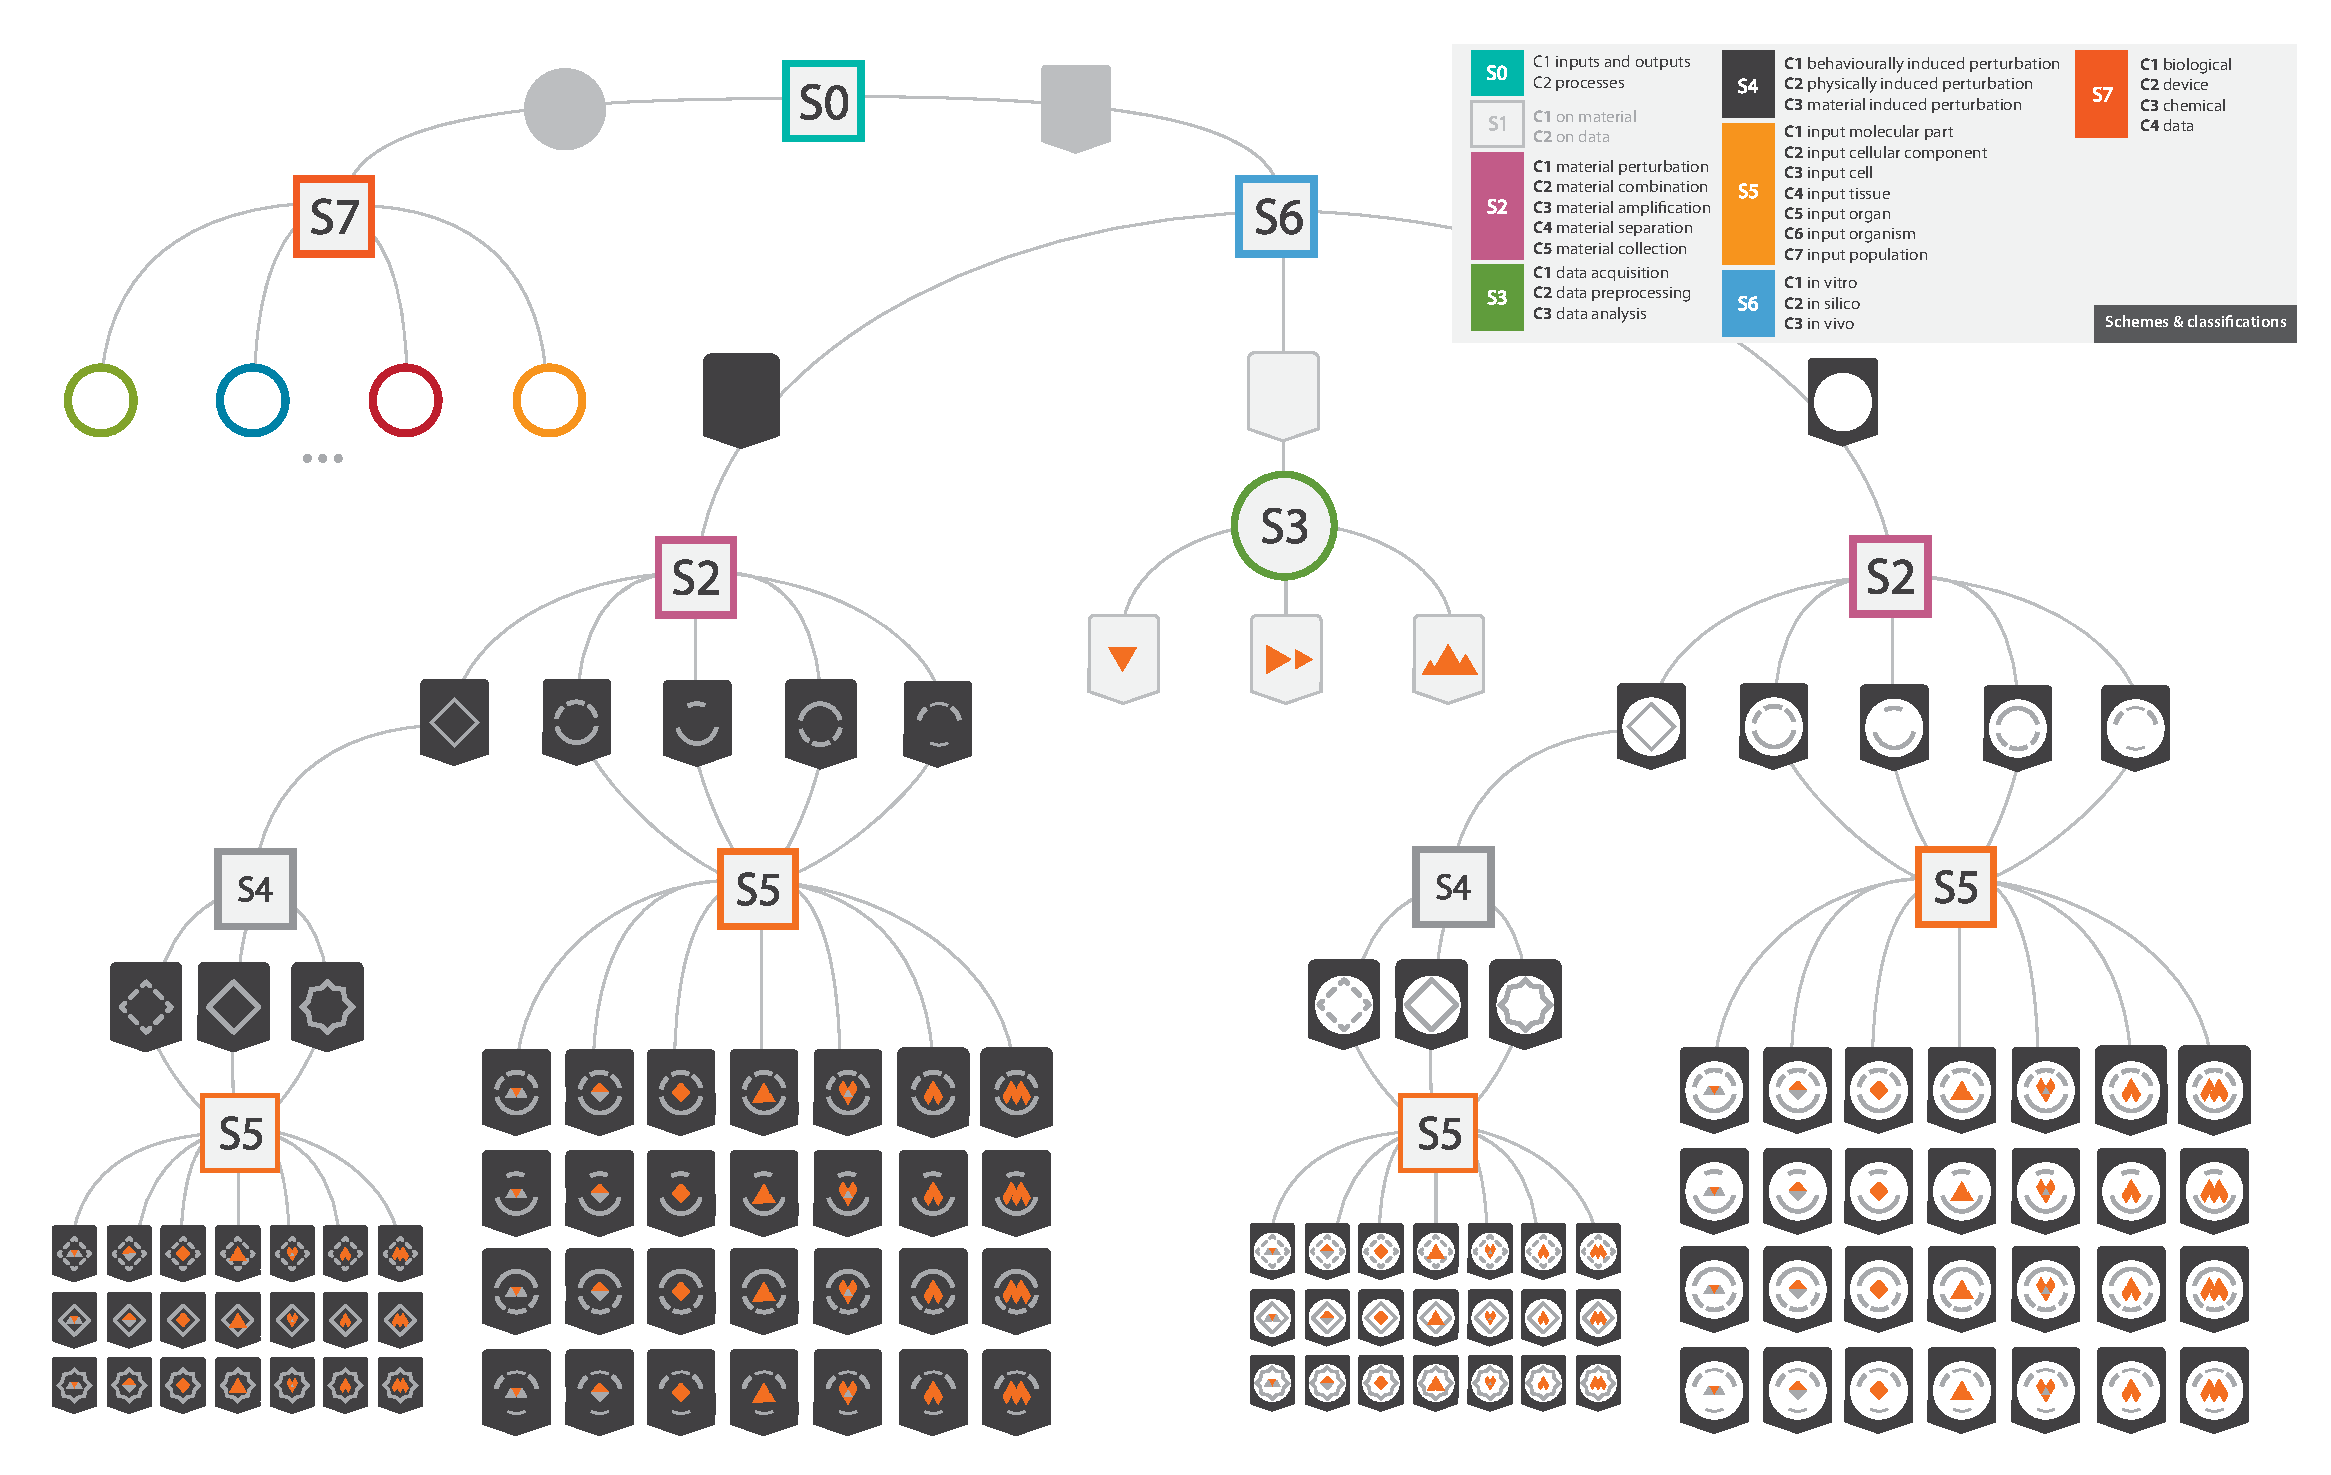
\includegraphics[scale=0.465]{images/glyph-taxonomy/full-tree.eps}
\caption{Overview of the taxonomy based glyph designs in the context of biodomain.}
\label{fig:full-tree}
\vspace{-5pt}
\end{figure*}

Following mapping of all schemes to design options, creation of all glyphs is a straightforward process.
Fig. \ref{fig:full-tree} shows all variations of the glyphs associated with the process sub-tree.

We introduced a ``crush'' test for the designed glyphs by scaling it to different pixel resolutions.
Fig. \ref{fig:crash-test} shows some example glyphs display at varying resolutions.
One can comfortably see all details at the 40$\times$40 level.
At the 10$\times$10 level, one can observe the visual signature of \emph{in vivo} and \emph{in vitro}.
Even at the lowest level (5$\times$5), one can still differentiate the two glyphs. 

\begin{figure}[t!]
\centering
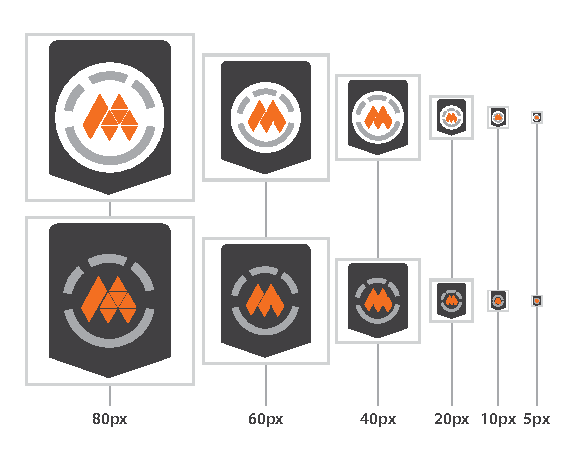
\includegraphics[scale=1]{images/glyph-taxonomy/crash-test.eps}
\caption{A ``crush'' test of glyphs to evaluate the discriminating capacity of various visual channels at different resolutions.}
\label{fig:crash-test}
\vspace{-5pt}
\end{figure}

% ===============
\section{Workflow Visualization and ISA Integration}
\label{sec:Workflow}

In order to visualize workflows of biological experiments, we had to address the following technical issues:
1) mapping from a name in the metadata to a glyph;
2) creating a workflow visualization with both node placement and connection display;
3) developing a prototype tool for a practical environment such as the ISA tools framework.

The mapping from concept name is achieved by a look-up table which is built from the matrix used in formulating the taxonomic tree and implemented as a tab delimited file.
Each concept name is mapped to a text tag encoding the traversal path from the root of the tree to the leaf node corresponding to the name.
The tag includes identifiers of the schemes and classes encountered.
With the path, a glyph can be constructed dynamically from the pre-defined visual mapping as described in the previous section.
The look-up table also enables storage of pre-rendered glyphs in an image format.

To generate the workflow, we made use of the layout algorithm available within the Prefuse visualization framework \cite{heer05}. This framework also brings with it functionality such as panning, zooming and filtering which bring more interactivity to the user and making navigation through large collections of workflows easier. The only requirement for use of Prefuse was a minimal amount of Java code to create the user interface coupled with creation of an XML file format native to Prefuse for representation of the tree structure. This XML format is configurable, we have configured it to contain: \emph{node type} (e.g., process), \emph{node
name} (e.g., labeling) and an image to be rendered, which is assigned using a look-up operation through the above mentioned tab delimited mapping file. The order of the XML elements within this file has direct implications on the order these elements are displayed in. Within the ISA-Tab format, there is an implicit time element found in the ordering of the columns in the study sample and assay files. This can be used to construct the XML elements through near direct mappings of processes and IOs, a workflow which is illustrated in Fig. \ref{fig:generating-workflow-from-text}. Recognizing branching events is an important part of workflow visualization as illustrated in \ref{fig:generating-workflow-from-text}. In software, these branch events can be identified when the preceding nodes of a process have the same names while the succeeding output nodes are different. Fig. \ref{fig:generating-workflow-from-text} highlights one such case, where branching occurs after extraction of 3 materials from one sample. 

Our software reads text-based ISA-Tab files as illustrated to create the XML notations required by Prefuse for rendering the experiment workflow illustrated in Fig. \ref{fig:teaser}(b).

\begin{figure}[t!]
\centering
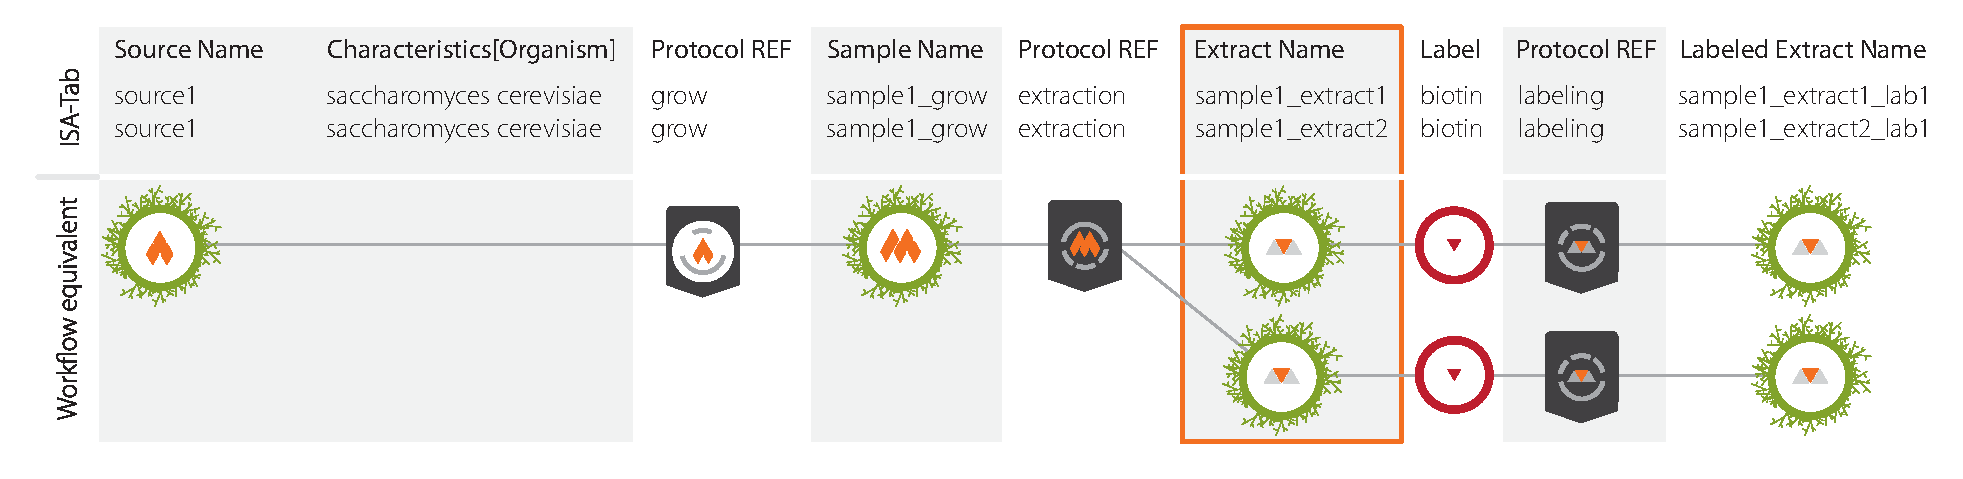
\includegraphics[scale=.2745]{images/glyph-taxonomy/generating-workflow-from-text.eps}
\caption{A workflow is recorded in text form within the ISA-Tab format.
Our software translates it to glyph-based visualization.
A branching event is automatically detected during the translation.}
\label{fig:generating-workflow-from-text}
\vspace{-10pt}
\end{figure}

\begin{figure}[ht!]
\centering
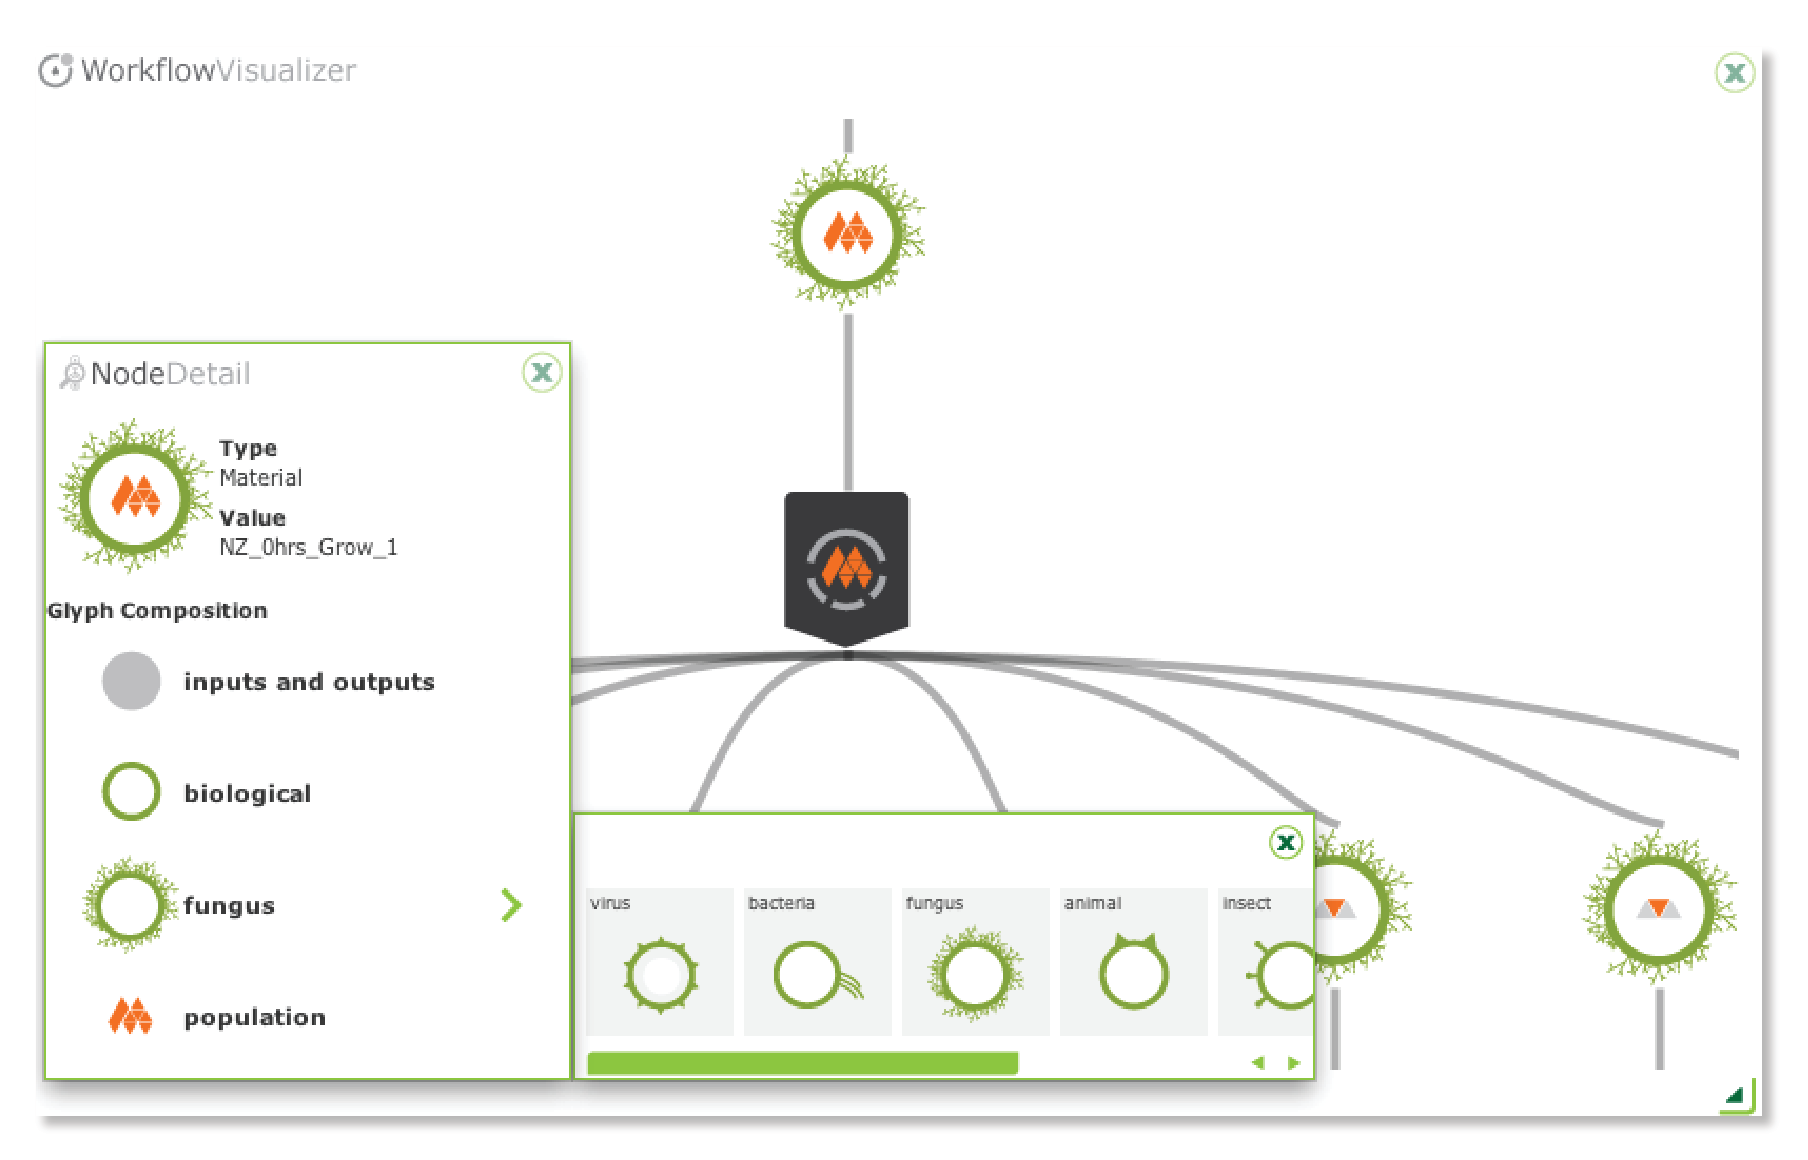
\includegraphics[scale=.295]{images/glyph-taxonomy/bio-workflow-example.eps}
\caption{User can interact with a workflow to view the text descriptions of individual glyphs in pop-up windows, which are also dynamic legends showing how the concept is categorized and how the corresponding glyph is decomposed into different elementary visual representations. Users can also use such a legend to find out other classes in a categorization scheme.}
\label{fig:bioworkflow-example}
\vspace{-15pt}
\end{figure}

The software is implemented as a Java application capable of processing ISA-Tab files to create experimental workflows using glyphs. For the purposes of broad dissemination in the near future, we have integrated the workflow visualization directly inside ISAcreator, a Java desktop application for creating and editing ISA-Tab files. Furthermore, the standalone workflow visualization shown in figures \ref{fig:bioworkflow-example}a and b makes use of the same ISA-Tab parser as available within ISAcreator. The integration involved the development of user interface elements for ISAcreator software to access the workflow visualization.
From the spreadsheet view, users may highlight rows (assays), right click and select an option named ``View workflow for assays'' to visualize the entire processing pipeline for the corresponding samples as shown in Fig. \ref{fig:teaser}(b).

\section{Conclusions and Future Work}
\label{sec:Conclusion}

Although it was established in psychology that people can learn rules of glyph encoding consciously as well as unconsciously \cite{franks71}, we do not expect users to learn and remember these glyphs without help. We thus allow users to find detailed text descriptions in pop-up windows interactively. As shown in Fig. \ref{fig:bioworkflow-example}, not only do these windows provide names of processes and IOs, they also serve as dynamic legends, showing how each glyph is decomposed into different elements corresponding to categorization schemes. One can also select a component to view all classes in a scheme.   

In this manuscript, we presented a systematic approach for glyph
design by using taxonomy as a guide. We demonstrated our approach by analyzing the content of a biological database and showed how our tree-building algorithm
could be used to take a large collection of concepts and generate a taxonomic tree, which
provides an ordering of a set of categorization schemes (i.e., attribute dimensions).
This enabled us to draw a parallel between the ordering of attribute dimensions with the ordering of visual channels compiled from the perception and visualization literature. 
We involved domain experts in refining the tree as well as in creating metaphoric abstraction and association for glyphs.
This work was followed by development of a prototype tool for glyph-based visualization of experimental design workflows as found in biology.
The prototype is integrated in the ISA suite of tools to be disseminated to users.

We plan to further the present work to include the provision of ``macros'' in workflows in order to make graphs more compact and create dynamic web-based rendering of the workflows using vector graphics.
We also intend to carry out field-based evaluation through ISAcommons, the user community of ISA-tools framework.
Like all potential diagrammatic schemes, we expect that it will take many iterations before it can become a standard.
Nevertheless, the development of an online visualization tool will make such a process more efficient.